
\subsection{Эмуляция работы кэша\footnote{Задача является дополнительной, желающие будут сдавать решение в систему автоматической проверки.}}

Необходимо проэмулировать работу $k$-way полностью ассоциативного кэша размера $cacheSize$ и с размером кэш-линии $lineSize$.

Для выполнения эмуляции будем:
\begin{itemize}
\item Обрабатывать адреса памяти один за одним, при этом считая, что каждый раз у нас запрашивается только один байт из памяти по данному адресу.
\item Изначально весь кэш пустует.
\item Если случается \texttt{CACHE\_MISS} и необходимо вытеснить одну из линий в кэше,
то будем вытеснять самую давно не используемую линию.
Т.е. в момент записи линии и в момент \texttt{CACHE\_HIT} ее внутренний счетчик времени выставляется в текущий момент.
\item Для определения номера кэш-линии необходимо разделить $address$ на $lineSize$ без остатка.
\item Для определения номера набора в кэше необходимо вычислить остаток от деления номера кэш-линии
на количество кэш-линий в одном банке памяти в кэше.
\end{itemize}

\begin{center}
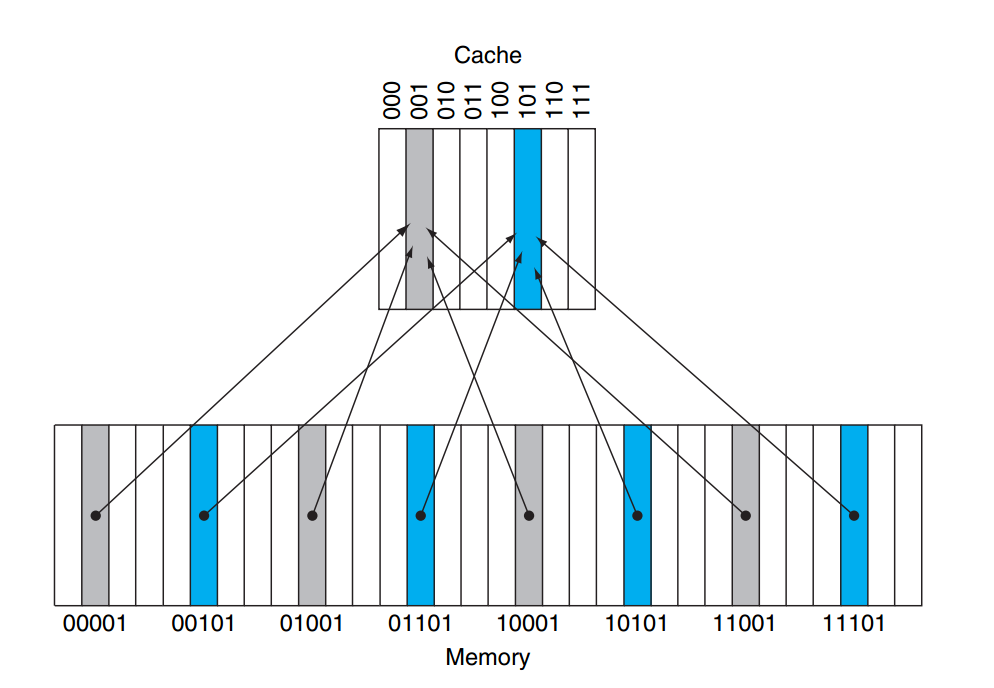
\includegraphics[scale=0.4]{images/cache.png}
\end{center}

В первой строке входных данных записаны четыре целых числа
$cacheSize$, $associativity$, $lineSize$ и $n$ ($2^{15} \le cacheSize \le 2^{24}$,
$associativity \in \{4,6,8,12,16\}$, $lineSize \in \{64, 128\}$, $1 \le n \le 100000$).

Вторая строка содержит $n$ целых чисел, последовательность адресов, к которым выполняется обращение.

Гарантируется:
\begin{itemize}
\item $cacheSize = associativity  \cdot 2^{k}$, для некоторого натурального $k$.
\item Все адреса в памяти из диапазона $[0; 2^{30} - 1]$.
\end{itemize}

Требуется выведите два числа, количество обращений к памяти, которые завершились \texttt{CACHE\_HIT} и
\texttt{CACHE\_MISS} соответственно.
